% -- Encoding UTF-8 without BOM
% -- XeLaTeX => PDF (BIBER)

\documentclass[]{cv-style}
\sethyphenation[variant=british]{english}{} % Add words between the {} to avoid them to be cut 

\begin{document}

\header{Ivan }{Khomutov}

%----------------------------------------------------------------------------------------
%	SIDEBAR SECTION  -- In the aside, each new line forces a line break
%----------------------------------------------------------------------------------------

\begin{aside}
%
\begin{tikzpicture}[x=\imagescale,y=-\imagescale]
    \clip (600/2, 567/2) circle (567/2);
    \node[anchor=north west, inner sep=0pt, outer sep=0pt] at (0,0) {%
        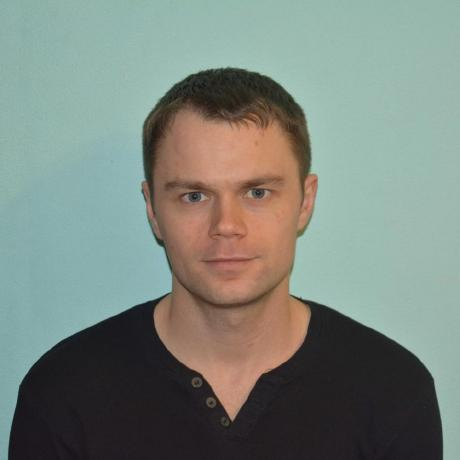
\includegraphics[width=\imagewidth]{photo.jpeg}%
    };
\end{tikzpicture}
%
\section{contacts}
\faMapMarker{} Saint Petersburg, Russia
~
\faMobilePhone{} +7 (911) 865 9112
~
\faEnvelope{} \href{mailto:iskhomutov@gmail.com}{iskhomutov@gmail.com}
~
\faGithub{} \href{http://github.com/iskhomutov}{iskhomutov}
%
\section{languages}
Russian mother tongue
English intermediate
%
\section{back-end}
Python, Django, Flask, Celery, pytest, fabric
%
\section{front-end}
ExtJS, BackboneJS, Marionette
%
\section{devops}
Git, PostgreSQL, Heroku
%
\section{misc}
Asterisk, Avaya, Telegram Bot API, 
%
\end{aside}

%----------------------------------------------------------------------------------------
%	SUMMARY SECTION
%----------------------------------------------------------------------------------------
\section{summary}

\begin{itemize}
%----------------------------------------------------------------------------------------
    \item Solid experience working with \textbf{Django} framework;
    \item Familiar with \textbf{Flask} framework;
    \item Experience in creating UI with various JS libraries: \textbf{Marionette}, \textbf{BackboneJS}, \textbf{ExtJS};
    \item Experience in writing REST like services using \textbf{django-rest-framework} and \textbf{spyne};
    \item Experience in real-time configuration and management of \textbf{PostgreSQL} database;
    \item Having experienced in \textbf{Agile} Methodologies;
    \item Knowledge in building Bots for the Telegram Messenger;
%----------------------------------------------------------------------------------------
\end{itemize}

%----------------------------------------------------------------------------------------
%	EXPERIENCE SECTION
%----------------------------------------------------------------------------------------
\section{experience}

\begin{entrylist}
%----------------------------------------------------------------------------------------
\entry
  {2017--Now}
  {Fogstream}
  {Khabarovsk, Russia}
  {\jobtitle{Full Stack Developer}\\
  Working as a developer in a medium-sized development team, that is primarily %
  responsible for the development and improvement of a variety of social services
  (Education, Agriculture, Employment). All of this services is based on a M3 framework,
  that is build upon Django and ExtJS. Demo of the project can be found
  at \href{http://school.bars-open.ru}{school.bars-open.ru}.

  Day-to-day responsibilities include:
  \begin{itemize}
      \item Developing the UI of the service, using \textbf{HTML}, \textbf{CSS}, \textbf{ExtJS} and \textbf{Jinja} templates;
      \item Implementing code to create dynamic xls reports, using \textbf{xlswriter} library;
      \item Building web services, using \textbf{spyne} library;
      \item Optimizing \textbf{PostgreSQL} queries;
      \item Refactoring legacy codebase;
      \item Writing unit tests;
      \item Adding docstrings for the current modules/classes/functions;
      \item Using \textbf{Git} version control system to coordinate team-development;
      \item Following Agile development methodology;
      \item Using Atlassian tools (\textbf{Jira/Stash/Confluence}) for developing;
      \item Attending daily meetings with other developers, analysts and QA testers.
  \end{itemize}}
%----------------------------------------------------------------------------------------
\entry
  {2013--2017}
  {Sberbank of Russia}
  {Khabarovsk, Russia}
  {\jobtitle{VoIP Engineer}\\
  Worked as a VOIP engineer, in the largest bank of the country. Started from the absolute zero with no practical knowledge in a such area.

  Main responsibilities:
  \begin{itemize}
      \item Administered and maintained Avaya 5.2 PBX system in the states head office with over3000 users;
      \item Installed, administered and maintained Avaya IP Office 406/500 PBX systems in a wide branch network (over 20 sites);
      \item Administered Avaya CMS with 100 agents;
      \item Administered and configured Asterisk PBX system, used as a auto-dial system;
      \item Managed Avaya SES, AES, Contact Recorder systems;
      \item Managed Cisco CUCM system;
      \item Installed and managed all sorts of phone endpoints;
  \end{itemize}}
%----------------------------------------------------------------------------------------
\end{entrylist}

%----------------------------------------------------------------------------------------
%	EDUCATION SECTION
%----------------------------------------------------------------------------------------
\section{education}

\begin{entrylist}
%----------------------------------------------------------------------------------------
\entry
{2007--2012}
{Bachelor {\normalfont in Telecommunications}}
{Far Eastern State Transport University (Khabarovsk, Russia)}
{\vspace{-0.3cm}}
\end{entrylist}
%----------------------------------------------------------------------------------------
\end{document}
